\documentclass{report}
\usepackage[
    % letterpaper,
    margin=1in,
    % headheight=13.6pt,
]{geometry}

%%%% Page Header and Foot %%%%
\usepackage{fancyhdr}
\fancypagestyle{plain}{
\fancyhf{}
\fancyhead[L]{ECE 14:332:226}
\fancyhead[C]{\textbf{Probability And Random Processes}}
\fancyhead[R]{Spring 2023}
\fancyfoot[L]{}
\fancyfoot[C]{\thepage}
\fancyfoot[R]{}
}
\pagestyle{plain}

%%%% Load Format %%%%
%%%% Page Margin %%%%
\RequirePackage{geometry}

%%%% Page Header and Foot %%%%
\RequirePackage{fancyhdr}
\pagestyle{fancyplain}
\lhead{\lefthead}
\chead{\centerhead}
\rhead{\righthead}
\lfoot{\leftbottom}
\cfoot{\centerbottom}
\rfoot{\rightbottom}

%%%% Additional Packages to Load %%%%
%%%% Main Font
\RequirePackage{lmodern} %Computer Modern, but with many more glyphs
\RequirePackage{microtype} %Better Font Rendering
\RequirePackage{libertinus} %Very popular math font
\RequirePackage[T1]{fontenc} %Better Printing Font
\RequirePackage[utf8]{inputenc} %enable utf8 encoding
\RequirePackage[english]{babel} %English Language

%%%% Math Env
\RequirePackage{amsfonts,amsmath,amssymb} %Math Font Packages
\RequirePackage{mathtools} %Better Math Environments
\RequirePackage{mleftright}  %Fixes some annoying spacing issues
\RequirePackage{bm} %Boldface math, load after other math font packages

%%%% Beautiful Stuff
\RequirePackage{graphicx} %Better Graphics
\RequirePackage[export]{adjustbox} %Better Graphics
\RequirePackage[dvipsnames,svgnames]{xcolor} %Must load before tcolorbox
\RequirePackage[breakable]{tcolorbox} %Customized Box
\tcbuselibrary{skins}
\RequirePackage{transparent} 

%%%% Table and List 
\RequirePackage{tabularx} %Better Table
\RequirePackage{multirow}
\RequirePackage{colortbl}
\RequirePackage{array}

%%%% Theorems etc (also  problems)
\RequirePackage[shortlabels]{enumitem} %Better List
\RequirePackage{hyperref, cleveref} %Fantastic crossrefer
\RequirePackage{amsthm, thmtools} %Better Theorems
\RequirePackage{thm-restate} %Better Theorems

%%%% Code Packages
\RequirePackage{algorithm2e} % Package to create pseudo-code
\RequirePackage{listings} % Package to insert code
% \RequirePackage{keyval}

%%%% Display Packages
\RequirePackage[document]{ragged2e} % Package to justify text
\RequirePackage{csquotes} % Package to facilities quotations
\RequirePackage{multicol} % Package to use multicols

%%%% Other Packages
\RequirePackage{calc}
\RequirePackage{rotating}
\RequirePackage{pgf, tikz}
\RequirePackage{epstopdf}
\RequirePackage[backend=biber, style=numeric, sorting=none]{biblatex}

%%%% A box fill the rest of the page
\newtcolorbox{stretchbox}[1][]{
    height fill,
    sharp corners,
    colback=white,
    % colframe=yellow!50!black,
    #1
    }

%%%% Box Environment
\newtcolorbox{prob}[1]{
% Set box style
    sidebyside,
    sidebyside align=top,
% Dimensions and layout
    width=\textwidth,
    toptitle=2.5pt,
    bottomtitle=2.5pt,
    righthand width=0.20\textwidth,
% Coloring
    colbacktitle=white,
    coltitle=black,
    colback=white,
    colframe=black,
% Title formatting
    title={
        #1 \hfill Grade:\hspace*{0.15\textwidth}
    },
    fonttitle=\large\bfseries
}

%%%% Problem Environment 
\newenvironment{problem}[1]{
    \begin{prob}{#1}
}
{
    \tcblower
    \centering
    \textit{\scriptsize\bfseries Faculty Comments}
    \end{prob}
}

%%%% Draw a line
\newcommand{\myrule}{\rule{1.5in}{0.1mm}}
%%%% delimiters
\DeclarePairedDelimiter\parens{\lparen}{\rparen}
\DeclarePairedDelimiter\bracks{\lbrack}{\rbrack}
\DeclarePairedDelimiter\braces{\lbrace}{\rbrace}
\DeclarePairedDelimiter\abs{\lvert}{\rvert}
\DeclarePairedDelimiter\norm{\lVert}{\rVert}
\DeclarePairedDelimiter\angles{\langle}{\rangle}
\DeclarePairedDelimiter\ceil{\lceil}{\rceil}
\DeclarePairedDelimiter\floor{\lfloor}{\rfloor}

%%%% math operators naming
\DeclareMathOperator*{\argmax}{\textnormal{argmax}}
\DeclareMathOperator*{\argmin}{\textnormal{argmin}}
\DeclareMathOperator{\tr}{\textnormal{tr}}
\DeclareMathOperator{\eig}{\textnormal{eig}}
\DeclareMathOperator{\sgn}{\textnormal{sgn}}
% \let\det\relax % "Undefine" \det
% \DeclareMathOperator{\det}{\textnormal{det}} % already defined in mathtools
\DeclareMathOperator{\diag}{\textnormal{diag}}
\DeclareMathOperator{\rank}{\textnormal{rank}}
\DeclareMathOperator{\Vol}{\textnormal{Vol}}   % volume
\DeclareMathOperator{\Surf}{\textnormal{Surf}} % surface area

%%%% Transforms! -- requires mathtools package
\newcommand*{\LapTrans}{\xleftrightarrow{\mathcal{Z}}}
\newcommand*{\ZTrans}{\xleftrightarrow{\mathcal{L}}}
\newcommand*{\CTFS}{\xleftrightarrow{\textnormal{CTFS}}}
\newcommand*{\CTFT}{\xleftrightarrow{\textnormal{CTFT}}}
\newcommand*{\DTFS}{\xleftrightarrow{\textnormal{DTFS}}}
\newcommand*{\DTFT}{\xleftrightarrow{\textnormal{DTFT}}}

%%%% vector font
\let\oldvec\vec
\renewcommand*{\vec}[1]{\mathbf{#1}}
% \newcommand*{\trn}{\!^{\!\intercal}}
\newcommand*{\trn}{\!^{\mathsf{T}}}
% \newcommand*{\coj}{\!^{\dag}} % Text Mode Symbol, Should not be used
% \newcommand*{\coj}{\!^{\dagger}}
\newcommand*{\coj}{\!^{\mathsf{H}}}
\newcommand*{\inv}{^{-1}}

%%%% number systems
\DeclareMathOperator{\R}{\mathbb{R}}
\DeclareMathOperator{\C}{\mathbb{C}}
\DeclareMathOperator{\N}{\mathbb{N}}
\DeclareMathOperator{\Z}{\mathbb{Z}}
\DeclareMathOperator{\F}{\mathbb{F}}
\DeclareMathOperator{\Q}{\mathbb{Q}}

%%%% STATISTICS AND PROBABILITY
\newcommand*{\Var}{\mathop{\textnormal{Var}}}
\newcommand*{\Cov}{\mathop{\textnormal{Cov}}}
\newcommand*{\Corr}{\mathop{\textnormal{Corr}}}
\newcommand*{\MSE}{\mathop{\textnormal{MSE}}}
\newcommand*{\MSD}{\mathop{\textnormal{MSD}}}
\newcommand*{\NSD}{\mathop{\textnormal{NSD}}}

\newcommand*{\E}[1]{\mathbb{E}\bracks*{#1}}
\newcommand*{\condE}[2]{\mathbb{E}\bracks*{#1 \mid #2}}
\renewcommand*{\P}[1]{\mathbb{P}\parens*{#1}}
\newcommand*{\condP}[2]{\mathbb{P}\parens*{#1 \mid #2}}

\DeclareMathOperator{\Bern}{\mathsf{Bern}}
\DeclareMathOperator{\Unif}{\mathsf{Unif}}
\DeclareMathOperator{\Expv}{\mathsf{Exp}}
\DeclareMathOperator{\Poi}{\mathsf{Poi}}
\DeclareMathOperator{\Gamv}{\mathsf{Gamma}}
\DeclareMathOperator{\Dirv}{\mathsf{Dir}}
\DeclareMathOperator{\Mult}{\mathsf{Mult}}
\DeclareMathOperator{\Beta}{\mathsf{Beta}}
\DeclareMathOperator{\Geomv}{\mathsf{Geom}}
\DeclareMathOperator{\Binomv}{\mathsf{Binom}}
\DeclareMathOperator{\NegBinomv}{\mathsf{NB}}
\DeclareMathOperator{\Lap}{\mathsf{Lap}}
\DeclareMathOperator{\Gaus}{\mathsf{N}}
\DeclareMathOperator{\Weibull}{\mathsf{Weibull}}


\DeclareMathOperator{\iidsim}{\stackrel{\textnormal{i.i.d.}}{\sim}}
\DeclareMathOperator{\diff}{\mathop{}\!\textnormal{d}}

%%%% Special norms and linear algebra stuff
\newcommand*{\subgnorm}[1]{\norm*{#1}_{\psi_2}}
\newcommand*{\subexpnorm}[1]{\norm*{#1}_{\psi_1}}
\newcommand*{\frobnorm}[1]{\norm*{#1}_{\textnormal{F}}}
\newcommand*{\opnorm}[1]{\norm*{#1}_{\textnormal{op}}}
\newcommand*{\Lipnorm}[1]{\norm*{#1}_{\textnormal{Lip}}}

%%%%
\newcommand*{\set}[1]{\braces*{\,#1\,}}
\newcommand*{\ie}{\textnormal{i.e.\ }}
\newcommand*{\eg}{\textnormal{e.g.\ }}
\newcommand*{\etc}{\textnormal{etc.\ }}
\newcommand*{\iid}{\textnormal{i.i.d.\ }}

%%%% Theorem Style %%%%
\declaretheorem[numbered=no, style=definition]{axiom}
\declaretheorem[numberwithin=chapter,style=definition]{definition}
\declaretheorem[sibling=definition]{theorem, lemma, corollary, proposition, conjecture}
\declaretheorem[numbered=no,style=remark]{remark, claim}

%%%% Document Information %%%%
\title{}
\author{}
\date{}

%%%% Start Document %%%%
% \geometry{
%     letterpaper,
%     top=1in,
%     bottom=1in,
%     inner=0.75in,
%     outer=0.75in
% }
\begin{document}
% \maketitle

\chapter{Set Theory, Probability, and Single Experiment}
\begin{enumerate}
    \item From Set to Probability (of the single experiment)
    \begin{enumerate}
        \item~{
            \begin{center}
                \begin{tabular}{|c|c|}
                    \hline
                    \textbf{Set Theory} & \textbf{Probability} \\
                    \hline
                    \hline
                    Element & Outcome \\
                    \hline
                    Subset  & Event   \\
                    \hline
                    Universal Set & Sample Space \\
                    \hline
                \end{tabular}
            \end{center}
                        }
            \item Outcome and Event: {
                \begin{enumerate}
                    \item Outcomes are always \textbf{Mutually Exclusive} since there are the smallest units (i.e., Elements) in the Set.
                    \item Event constitutes by different combinations of outcomes (through Union ($\cup$) Operation).
                \end{enumerate}
            } 
            \item $\P{\text{Event}}$ is the possibility that the event appears in the sample space. 
            \item $\P{\emptyset}=0$ since there is no element in \textit{null set}, and $\P{\text{Sample Space}}=1$.
    \end{enumerate}
    \item From Set Operation to Probability Operation
    \begin{enumerate}
        \item There are three Set Operations: $A \cup B, A \cap B, A^{^\mathsf{c}}$.
        \item $\P{A \cup B} = \P{A}+\P{B}-\P{A\cap B}$.
        \item \textbf{Union Bound:} $\P{\cup_{i=1}^N A_i}\leq \sum_{i=1}^{N}\P{A_i}$.
        \item \textbf{Mutually Exclusive:}~$\P{A \cap B}=0$ so that $\P{A \cup B} = \P{A}+\P{B}$.
        \item \textbf{Collectively Exhaustive:}~$\P{A\cup B}=1$.
        \item \textbf{Partitions (i.e., Mutually Exclusive \& Collectively Exhaustive):}~$\P{\cup_{i=1}^N A_i}=\sum_{i=1}^{N}\P{A_i}=1$.
    \end{enumerate}
    \item Conditional Probability
    \begin{enumerate}
        \item $\condP{A}{B} = \frac{\P{AB}}{\P{B}}$.
        \item \textbf{If $A_i$ are Mutually Exclusive:}~$\condP{A}{B} = \condP{\cup_{i=1}^{N}A_i}{B} = \sum_{i=1}^{N}\condP{A_i}{B}$.
        \item \textbf{If $B_i$ are Partitions}~(Law of Total Number),
        \begin{align}
             \condP{A}{B} 
             &= \frac{\P{AB}}{\P{B}}  \tag{Definition of Conditional Probability}\\
             &= \P{AB}  \tag{$B$ is Collectively Exhaustive so $P(B)=1$} \\
             &= \P{A\cdot\cup_{i=1}^{N}B_i}  \tag{$B$ is Mutually Exclusive} \\
             &= \sum_{i=1}^{N}\P{AB_i}  \tag{$B$ is Partition} \\
             &= \sum_{i=1}^{N}\condP{A}{B_i}\P{B_i}. \tag{Definition of Conditional Probability}
        \end{align}
    \end{enumerate}
    \item Bayes' Theorem:~$\condP{A}{B} = \frac{\condP{B}{A}\P{A}}{\P{B}}$.
    \item Independent:{
        \begin{enumerate}
            \item $\P{A\cap B}=\P{A}\P{B}$.
            \item $\P{A \cup B} = \P{A}+\P{B}-\P{A}\P{B}$.
            \item $\condP{A}{B} = \frac{\P{AB}}{\P{B}}=\frac{\P{A}\P{B}}{\P{B}}=\P{A}$.
        \end{enumerate}
    } 
\end{enumerate}
\section*{Chapter 2: Sequential Experiments}
\begin{enumerate}
    \item Tree Diagrams
    \item Counting Methods (\textbf{Essentially the outcomes in each experiment (i.e., sample space) are equiprobable})
    \begin{enumerate}
        \item Multiplication:~$n\times k_1\times k_2\times \ldots$
        \item Sampling without Replacement
        \begin{enumerate}
            \item Permutation:~$\frac{n!}{(n-k)!}$.
            \item Combination:~$\binom{n}{k}=\frac{n!}{k!(n-k)!}=\binom{n}{n-k}$.
            \item Combination is Permutation without order. Combination is also called n choose k.
        \end{enumerate}
        \item Sampling with Replacement:~$n^k$
        \item Multiple Combination:{
            \begin{enumerate}
                \item $\binom{n}{k_1,k_2,\ldots,k_m}=\frac{n!}{k_1!k_2!\ldots k_m!}$ where $n=\sum_{i=1}^{m}k_i$
                \item For the two cases situation, $n=k_1+k_2\iff \binom{n}{k_1k_2}=\frac{n!}{k_1!k_2!}\iff\binom{n}{k_1}\iff\binom{n}{k_2}$
            \end{enumerate}
            }
    \end{enumerate}
    \item Independent Trails (\textbf{Essentially the outcomes in each sample space are not necessarily equiprobable})
    \begin{enumerate}
        \item \textit{Theorem 2.8:} The Probability of $k_0$ failures and $k_1$ successes in $n=k_0+k_1$ Independent Trails with success rate $p$ is \[\P{k_0, k_1}=\binom{n}{k_0}(1-p)^{k0}p^{k_1}=\binom{n}{k_1}(1-p)^{k0}p^{k_1}\]
        \item \textit{Theorem 2.9:} $n=k_1+k_2+\ldots+k_m$ and success rates are $p_1, p_2,\ldots,p_m$, where $\sum_{i=1}^{m}p_i=1$ has 
        $$P(k_1,k_2,\ldots,k_m)=\binom{n}{k_1,k_2,\ldots,k_m}p_1^{k_1}p_2^{k_2}\ldots p_m^{k^m}.$$
        % \item If the outcomes in each sample space is equiprobable, the question can be solved by Sampling with Replacement.
    \end{enumerate}
\end{enumerate}
\section*{Chapter 3: Discrete Random Variables}
\begin{enumerate}
    \item Discrete Random Variables: Assign numerical value to discrete outcomes
    \item Probability Mass Function~(PMF): $$\sum_{x\in X}P_X(x)=1$$ 
    \item Families of Discrete Random Variables and their PMF{
        \begin{enumerate}
            \item Bernoulli(p): \textbf{E.g., Flip a coin}{
                \[ P_X(x) = 
                \begin{cases}
                    1-p & x=0, \\
                    p   & x=1, \\
                    0   & otherwise.
                \end{cases} \]
            }
            \item Binomial(n,p): Get \textbf{x} successes in \textbf{n} Bernoulli(p) experiments $\iff$ independent trails{
                $$P_X(\textcolor{red}{x}) = \binom{n}{\textcolor{red}{x}}p^x(1-p)^{n-x}$$.
            }
            \item Poisson($\alpha$): Binomial(n,p) with extremely small p (a.k.a. $\alpha$) and large n{
                \[ P_X(x) = 
                \begin{cases}
                    \dfrac{\alpha^xe^{-\alpha}}{x!}   & x=0,1,\ldots \\
                    0   & otherwise.
                \end{cases} \]
            }
            \item Geometric(p): Get the \textbf{1st} success at the \textbf{x-th} Bernoulli(p) experiment {
                \[ P_X(x) = 
                \begin{cases}
                    p(1-p)^{x-1} & x=1,2,\ldots \\
                    0   & otherwise.
                \end{cases} \]
            }
            \item Pascal(k,p): Get the \textbf{k-th} success at the \textbf{x-th} Bernoulli(p) experiment (Geometric(p) is Pascal(1,p)){
                $$P_X(\textcolor{red}{x}) = \binom{\textcolor{red}{x-1}}{k-1}p^k(1-p)^{x-k}$$.
            }
            \item Discrete Uniform(k,l): outcomes are uniformly distributed on range (k,l) \textbf{E.g., Roll a Dice}{
                \[ P_X(x) = 
                \begin{cases}
                    1/(l-k+1)   & x=k,k+1,k+2,\ldots,l \\
                    0   & otherwise.
                \end{cases} \]
            }            
        \end{enumerate}
    }
    \item Cumulative Distribution Function~(CDF): {
        \begin{align*}
            F_X(x)&=P_X[X\leq x] \\
            F_X(b)-F_X(a)&=P_X(a<X\leq b)
        \end{align*}
    }
    \item Average and Expectations{
        \begin{enumerate}
            \item In ordinary language, an \textbf{Average} is a single number taken as representative of a list of numbers.{
            \begin{enumerate}
                \item Mode: The outcome appears the most often in the sample space $$P_X(x_{mod})\geq P_X(x)$$
                \item Median: The outcome which separates the higher half from  the lower half of a sample space $$P[X\leq x_{med}]\geq 1/2 \qquad \qquad P[X\geq x_{med}]\geq 1/2$$
                \item (Arithmetic) mean:  The sum of all the outcomes divided by the number of outcomes $$\bar{x} = \frac{1}{n}\sum_{i=1}^{n}x_i$$
            \end{enumerate}
            }
            \item Expectations: Weighted (Arithmetic) mean{
                \begin{enumerate}
                    \item Definition:{
                        \begin{align}
                            \mu_x = \E{X}&=\sum_{x\in S_X}xP_X(x) \tag{First Moment of $X$}\\
                            \E{X^2}&=\sum_{x\in S_X}x^2P_X(x) \tag{Second Moment of $X$}
                        \end{align}
                    }
                    \item Important Expectations{
                        \begin{enumerate}
                            \item Bernoulli(p): $$\E{X}=0\cdot P_X(0)+1\cdot P_X(1)=0(1-p)+1(p)=p$$
                            \item Binomial(n,p): $$\E{X}=np$$
                            \item Poisson($\alpha$): $$\E{X}=\alpha$$
                            \item Geometric(p): $$\E{X}=\sum_{x=1}^{\infty}xP_X(x)=\sum_{x=1}^{\infty}xp(1-p)^{x-1}=\dfrac{p}{1-p}\sum_{x=1}^{\infty}x(1-p)^x=\dfrac{p}{1-p}\dfrac{1-p}{[1-(1-p)]^2}=\dfrac{p}{p^2}=\dfrac{1}{p}$$
                            \item Pascal(k,p): $$\E{X}=k/p$$
                            \item Discrete Uniform(k,l): $$\E{X}=(k+l)/2$$
                        \end{enumerate}
                    }
                \end{enumerate}
            }
        \end{enumerate}
    }
    \item Derived Random Variable: $Y = g(X)${
        \begin{enumerate}
            \item $P_Y(y) = P[Y=y] = P[Y=g(x)] = P[g^{-1}(Y)=g^{-1}(g(x))] = P[X=x] = P_X(x)$
            \item $\E{Y} = \sum yP_Y(y) = \sum g(x)P_X(x)$
            \item $\E{X-\mu_x}=\sum_{x\in S_X}(x-\mu_x)P_X(x)=\sum_{x\in S_X}xP_X(x)-\mu_x\sum_{x\in S_X}P_X(x)=\E{X}-\mu_x\cdot 1=\mu_x-\mu_x=0$
            \item $\E{aX+b}=a\E{X}+b \Rightarrow \E{b}=\E{0\cdot X+b}=b$
        \end{enumerate}
    }
    \item Variance($\sigma_x^2$) and Standard Deviation($\sigma_x$){
        \begin{enumerate}
            \item $\sigma_x^2=\Var(X)$ $$\Var(X)=\E{(X-\mu_x)^2}=\E{X^2-2\mu_xX+\mu_x^2}=\E{X^2}-2\mu_x\E{X}+\E{\mu_x^2}=\E{X^2}-2\mu_x^2+\mu_x^2=\E{X^2}-\mu_x^2$$
            \item $\Var(X)\geq 0$
            \item $\Var(aX+b)=a^2\Var(X)$
            \item Important Variance:{
                \begin{enumerate}
                    \item Bernoulli(p): $$\Var(X)=p(1-p)$$
                    \item Binomial(n,p): $$\Var(X)=np(1-p)$$
                    \item Poisson($\alpha$): $$\Var(X)=\alpha$$
                    \item Geometric(p): $$\Var(X)=(1-p)/p^2$$
                    \item Pascal(k,p): $$\Var(X)=k(1-p)/p^2$$
                    \item Discrete Uniform(k,l): $$\Var(X)=(l-k)(l-k+2)/12$$
                \end{enumerate}
            }
        \end{enumerate}
    }
\end{enumerate}
\chapter{Continuous Random Variables}


\section{Continuous sample space}
\begin{axiom}
    A random variable $X$ is continuous if the sample space $S_X$ consists of one or more intervals. For $x\in S_X$, $P_X(x)=0$.
\end{axiom}


\section{The Cumulative Distribution Function}
\begin{definition}[Cumulative Distribution Function (CDF)]
    The CDF of continuous random variable $X$ is
    \[F_X(x) = \P{X\leq x}.\]
\end{definition}

\begin{theorem}
    For any random variable $X$,
    \begin{enumerate}
        \item $F_X(-\infty)=0$
        \item $F_X(\infty)=1$
        \item $\P{x_1<X\leq x_2} = F_X(x_2)-F_X(x_1)$
    \end{enumerate}
\end{theorem}


\section{Probability Density Function}
Start with a continuous random variable $X$ with CDF $F_X(x)$. The probability of ``$X$ with volume $\triangle$'' is defined as:
\begin{align*}
    \P{x<X\leq x+\triangle}
    &= F_X(x+\triangle)-F_X(x) \\
    &= \frac{F_X(x+\triangle)-F_X(x)}{(x+\triangle)-x}\cdot\triangle.
\end{align*}
\begin{definition}[Probability Density Function (PDF)]
    \begin{align*}
        f_X(x)
        &= \lim_{\triangle\rightarrow 0}\frac{F_X(x+\triangle)-F_X(x)}{\triangle} \\
        &= \frac{\diff F_X(x)}{\diff x}.
    \end{align*}
\end{definition}

\begin{theorem}
    For a continuous random variable $X$ with PDF $f_X(x)$,
    \begin{enumerate}
        \item $f_X(x)\geq 0$ for all $x$
        \item $F_X(u)=\int_{-\infty}^u f_X(x)\diff x$
        \item $\int_{-\infty}^{\infty} f_X(x)\diff x = 1$
    \end{enumerate}
\end{theorem}

\begin{theorem}
    \begin{align*}
        \P{x_1<X\leq x_2}=\int_{x_1}^{x_2}f_X(x)\diff x.
    \end{align*}
\end{theorem}


\section{Expected Value}
\begin{definition}[Expected value]
    \begin{align*}
        \E{X}=\int_{-\infty}^{\infty} xf_X(x) \diff x.
    \end{align*}
\end{definition}

\begin{corollary}
    [Integral Identity]
    For every non-negative random variable $X$, \[\E{X}=\int_{0}^{\infty}1-F_X(u)\diff s=\int_{0}^{\infty}\P{X>u}\diff u.\]

\end{corollary}

\begin{theorem}[Derived Random Variable]
    \begin{align*}
        \E{g(X)} = \int_{-\infty}^{\infty} g(x)f_X(x)\diff x.
    \end{align*}
\end{theorem}

\begin{theorem}
    For any random variable $X$,
    \begin{enumerate}
        \item $\E{X-\mu_x}=0$,
        \item $\E{aX+b}=a\E{X}+b$,
        \item $\Var[X] = \E{X^2}-\mu_x^2$,
        \item $\Var[aX+b]=a^2\Var[X]$.
    \end{enumerate}
\end{theorem}

\section{Families of Continuous Random Variables}
\begin{enumerate}
    \item Continuous Uniform $(k,l)$: A continuous counterpart of Discrete Uniform {
        \begin{align*}
            f_X(x)
            &= {
                \begin{cases}
                \frac{1}{l-k} & k\leq x \leq l \\
                0             & otherwise.
                \end{cases} } \\
            F_X(x)
            &= \frac{x-k}{l-k}. \qquad x\in (k,l)\\
            \E{X}
            &= (l+k)/2. \\
            \Var[X]
            &= (l-k)^2/12. \\
        \end{align*}
    }
    \item Exponential $(\lambda)$: A continuous counterpart of Geometry $(1-e^{-\lambda})$ {
        \begin{align*}
            f_X(x)
            &= {
                \begin{cases}
                    \lambda e^{-\lambda x} & x\geq 0 \\
                    0                      & otherwise.
                \end{cases}
            } \\
            F_X(x)
            &= 1-e^{-\lambda x}. \\
            \E{X}
            &= 1/\lambda. \\
            \Var[X]
            &= 1/\lambda^2.
        \end{align*}
    }
    \item Erlang $(n,\lambda)$: A continuous counterpart of  $(n,1-e^{-\lambda})${
        \begin{align*}
            f_X(x)
            &= {
                \begin{cases}
                    \frac{\lambda (\lambda x)^{n-1}e^{-\lambda x}}{(n-1)!} & x\geq 0 \\
                    0      & otherwise.
                \end{cases}
            } \\
            F_X(x)
            &= 1-\sum_{k=0}^{n-1}\frac{(\lambda x)^k e^{-\lambda x}}{k!} = \mathbb{P}_{\mathbf{poisson}}(k\geq n). \\
            \E{X}
            &= n/\lambda. \\
            \Var[X]
            &= n/\lambda^2.
        \end{align*}
    }
\end{enumerate}


\section{Gaussian Random Variables}
\begin{theorem}[Gaussian Integral]
    \[\int_{-\infty}^{\infty}e^{-x^2}\diff x=\sqrt{\pi}.\]
\end{theorem}

\begin{definition}[Gaussian Random Variable]
    $X$ is a $\mathsf{Gaussian}(\mu, \sigma)$ random variable if the \textrm{PDF} of $X$ is
    \[f_X(x)=\frac{1}{\sqrt{2\pi\sigma^2}}\exp(-\frac{(x-\mu)^2}{2\sigma^2}).\]
    $X$ is also called $\mathsf{Normal}(\mu,\sigma)$ random variable. We will use $\mathsf{N}(\mu, \sigma)$ in the following content.
\end{definition}

\begin{theorem}[The Expectation and Variance of $X\sim\Gaus(\mu,\sigma)$]
    \[\E{X} = \mu, \qquad \Var[X] = \sigma^2.\]
\end{theorem}

\begin{theorem}
    If $X$ is $\Gaus(\mu,\sigma)$, $Y=aX+b$ is $\Gaus(a\mu+b,a\sigma)$.
\end{theorem}

\begin{theorem}[Standard Normal Random Variable]
    The $\Gaus(\mu,\sigma)$ with $\mu=0, \sigma=1$ is called standard normal random variable $Z\sim\Gaus(0,1)$. The \emph{PDF} is,
    \[f_X(x)=\frac{1}{\sqrt{2\pi}}\exp(-\frac{x^2}{2}).\]
    And the \emph{CDF} is
    \[\Phi(z)=\int_{-\infty}^{z}\frac{1}{\sqrt{2\pi}}\exp(-\frac{x^2}{2})\diff x.\]
\end{theorem}

\begin{theorem}
    If $X$ is $\Gaus(\mu,\sigma)$, the \emph{CDF} of $X$ is
    \[F_X(x)=\Phi\parens*{\frac{x-\mu}{\sigma}}.\]
    The probability that $X$ is in the interval \emph{$(a,b)$} is
    \[\P{a<X\leq b}=\Phi\parens*{\frac{b-\mu}{\sigma}}-\Phi\parens*{\frac{a-\mu}{\sigma}}.\]
\end{theorem}

\begin{theorem}
    $\Phi(-z)=1-\Phi(z)$.
\end{theorem}

% 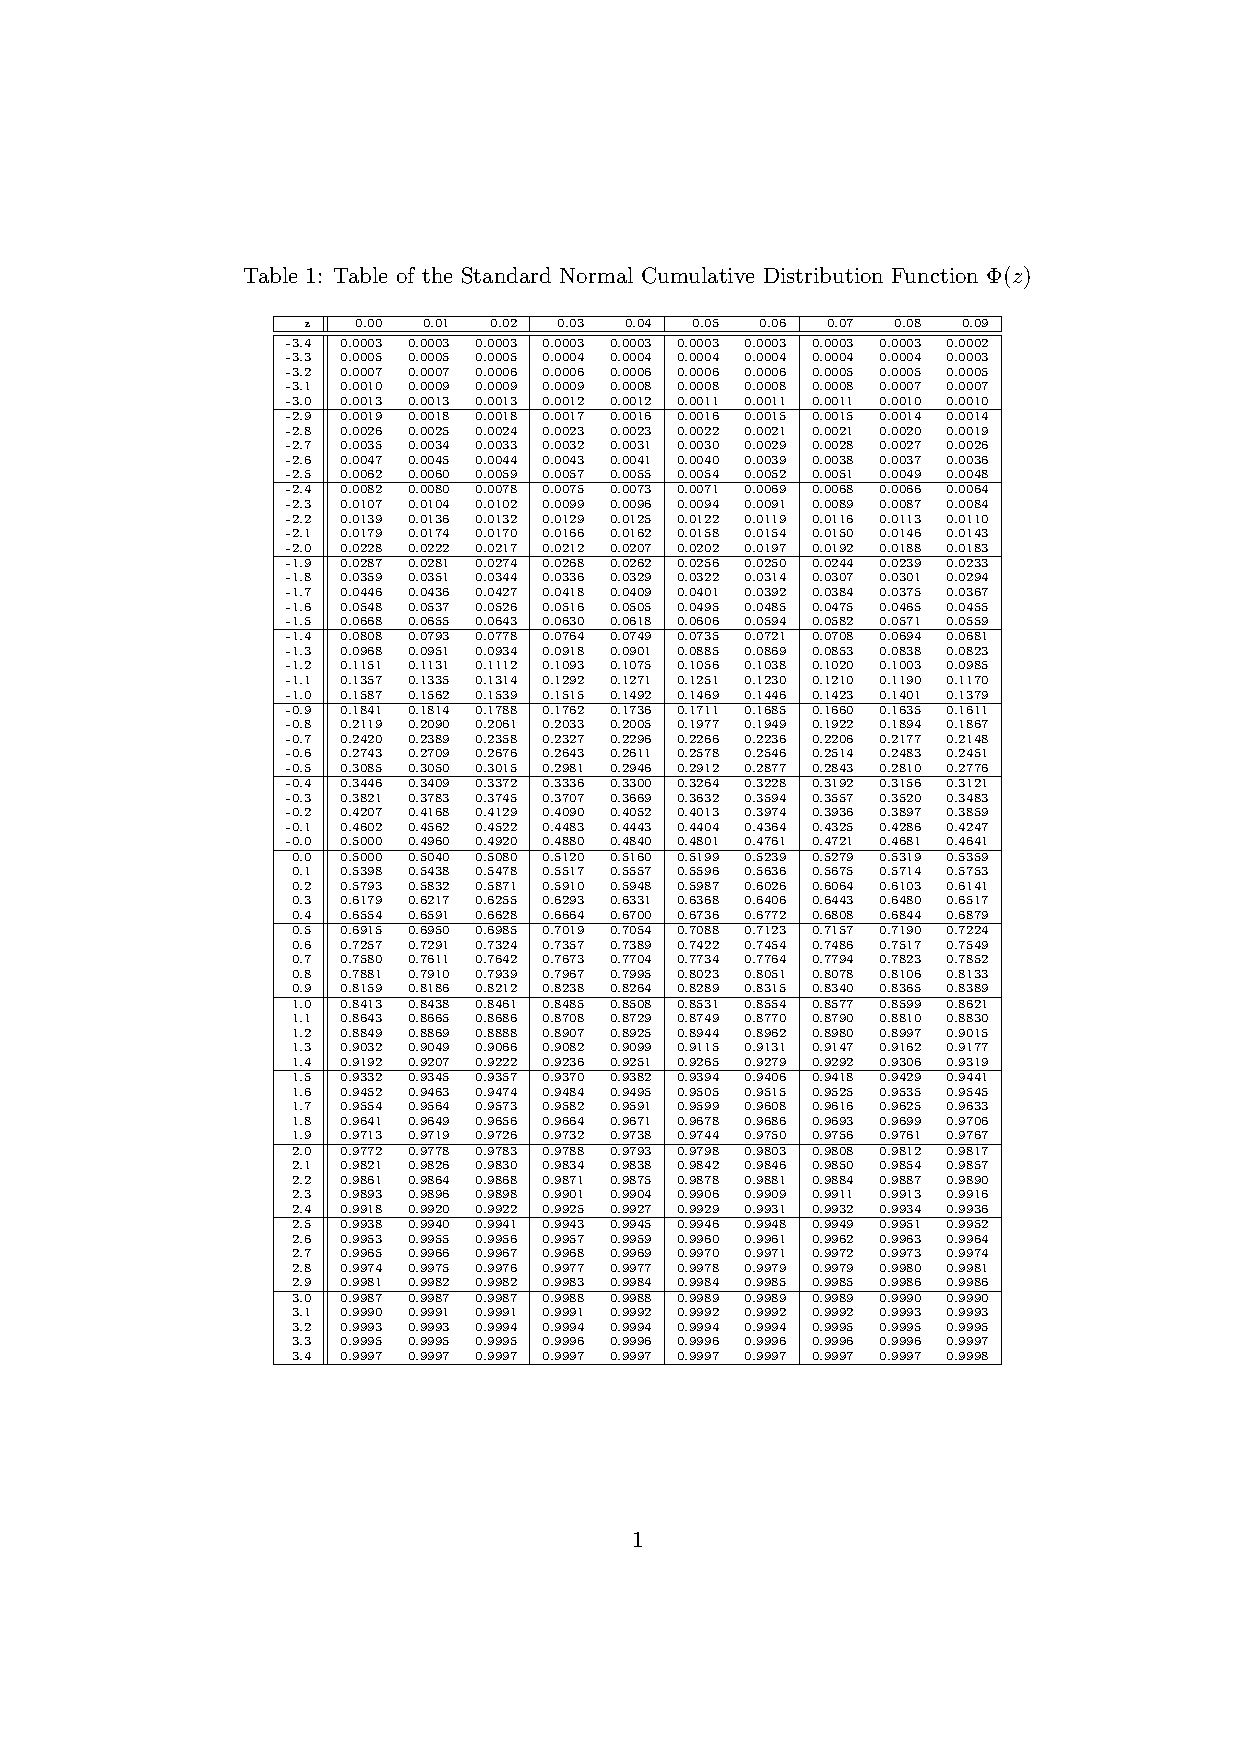
\includegraphics[width=\textwidth, center]{normal_cdf.pdf}

\section{Delta Function, Mixed (Being Discrete and Continuous at the same time) Random Variable}
\begin{definition}[Unit Impulse (Delta) Function]
    Let
    \[d_{\epsilon}(x)={
        \begin{cases}
            1/\epsilon & -\epsilon/2\leq x\leq \epsilon/2 \\
            0 & otherwise.
        \end{cases}
    }\]
    The \textbf{unit impulse function} is
    \[\delta(x)=\lim_{\epsilon\rightarrow 0}d_{\epsilon}(x).\]
    Since
    \[\int_{-\infty}^{\infty}\delta(x)\diff x = 1.\]
    The $\delta(x)$ is indeed a PDF given it is also non-negative.
\end{definition}

\begin{theorem}
    For any continuous function $g(x)$,
    \[\int_{-\infty}^{\infty}g(x)\delta(x-x_0)\diff x = g(x_0).\]
\end{theorem}

\begin{definition}[Unit Step Function]
    The \textbf{unit step function} is
    \[u(x)={
        \begin{cases}
            0 & x<0, \\
            1 & x\geq 0.
        \end{cases}
    }\]
\end{definition}

\begin{theorem}[CDF of $\delta(x)$ and connection to the unit step function]\label{delta}
    \[\int_{-\infty}^{x}\delta(v)\diff v = u(x).\]
    And thus
    \[\delta(x)=\frac{\diff u(x)}{\diff x}.\]
\end{theorem}

\begin{corollary}
    The~\cref{delta} allows us to define a generalized \emph{PDF} that applies to discrete random variables as well as to continuous random variables. Consider the \emph{CDF} of a discrete random variable, $X$. It is constant (let's say $0$ for now) everywhere except at point $x_i\in S_X$, where it has jumps of height $P_X(x_i)$. Using the \textbf{unit step function}, the \emph{CDF} of $X$ is
    \[F_X(x)=\sum_{x_i\in S_X} P_X(x_i)u(x-x_i).\]
    And the \emph{PDF} can be defined with $\delta(x)$ as
    \[f_X(x)=\sum_{x_i\in S_X}P_X(x_i)\delta(x-x_i).\]
    Then the \emph{Expectation} will be
    \begin{align*}
        \E{X} &= \int_{-\infty}^{\infty}x\sum_{x_i\in S_X}P_X(x_i)\delta(x-x_i)\diff x \\
        \E{X} &= \sum_{x_i\in S_X}\int_{-\infty}^{\infty}xP_X(x_i)\delta(x-x_i)\diff x \\
        &= \sum_{x_i\in S_X}x_i P_X(x_i)
    \end{align*}
\end{corollary}

\begin{theorem}
    For a random variable $X$ (not specified whether it is discrete or continuous), we have
    \begin{align*}
        q
        &= \P{X=x_0} && \text{(General expression)} \\
        &= P_X(x_0) && \text{(PMF)} \\
        &= F_X(x_0^+) - F_X(x_0^-) && \text{(CDF)} \\
        &= f_X(x_0) = q\delta(0). && \text{(PDF \& delta function)}
    \end{align*}
\end{theorem}

\begin{theorem}
    $X$ is a \textbf{mixed} random variable if and only if $f_X(x)$ contains both impulses and nonzero, finite values.
\end{theorem}
\chapter{Multiple Random Variables}

\section{Joint CDF}
\begin{definition}[Joint CDF]
    The joint CDF of random variables $X$ and $Y$ is 
    \[F_{X,Y}(x,y) = \P{X\leq x, Y\leq y}.\]
\end{definition}

The joint CDF is a \textbf{complete} probability model for any pair of random variables $X$ and $Y$.

\begin{theorem}
    For any pair of random variables, $X$ and $Y$, the following properties hold:
    \begin{enumerate}[(a)]
        \item $0 \leq F_{X,Y}(x,y) \leq 1$,
        \item $F_{X,Y}(\infty,\infty)=1$,
        \item $F_{X,Y}(-\infty,y)=F_{X,Y}(x,-\infty)=0$,
        \item $F_X(x)=F_{X,Y}(x,\infty)$ and $F_Y(y)=F_{X,Y}(\infty,y)$,
        \item $F_{X,Y}(x,y)$ is non-decreasing in $x$ and $y$.
    \end{enumerate}
\end{theorem}

\section{Joint PMF}
\begin{definition}[Joint PMF]
    The joint PMF of random variables $X$ and $Y$ is 
    \[P_{X,Y}(x,y) = \P{X=x, Y=y}.\]    
\end{definition}

The joint PMF is a \textbf{complete} probability model for any pair of discrete random variables $X$ and $Y$.

\begin{theorem}
    For discrete random variables $X$ and $Y$ and any set $B$ in the $X$, $Y$ plane, the probability of the event 
    % $\set{(X,Y)\in B}$ 
    is 
    \[\P{[B]}=\sum_{(x,y)\in B}P_{X,Y}(x,y).\]
\end{theorem}

Apparently, the joint PMF is non-negative and sums to one.
\[\sum_{x\in S_X}\sum_{y\in S_Y}P_{X,Y}(x,y)=1.\]

\section{Marginal PMF}
\begin{theorem}
    For discrete random variables $X$ and $Y$ with joint PMF $P_{X,Y}(x,y)$, 
    \[P_X(x)=\sum_{y\in S_Y}P_{X,Y}(x,y), \qquad P_Y(y)=\sum_{x\in S_X}P_{X,Y}(x,y).\]
\end{theorem}
For discrete random variables, the marginal PMF $P_X(x)$ and $P_Y(y)$ are probability models for the individual random variables $X$ and $Y$, but they only provide an \textbf{incomplete} probability model for the pair of random variables $X$ and $Y$.

\section{Joint PDF}
\begin{definition}[Joint PDF]
    The joint CDF of continuous random variables $X$ and $Y$ is a function $f_{X,Y}(x,y)$ with the property
    \[F_{X,Y}(x,y)=\int_{-\infty}^{x}\int_{-\infty}^{y}f_{X,Y}(u,v)\diff u \diff v.\]
\end{definition}

Apparently, we can then derive the joint PDF as follows,
\[f_{X,Y}(x,y)=\frac{\partial^2}{\partial x \partial y}F_{X,Y}(x,y).\]
The joint PDF is a \textbf{complete} probability model for any pair of continuous random variables $X$ and $Y$.

\begin{theorem}
    The probability that the continuous random variables $(X,Y)$ are in $A$ 
    \[\P{[A]}=\iint\limits_A f_{X,Y}(x,y)\diff x\diff y.\]
\end{theorem}

The joint PDF is non-negative and integrates to one.
\[\int_{-\infty}^{\infty}\int_{-\infty}^{\infty}f_{X,Y}(x,y)\diff x\diff y=1.\]

\section{Marginal PDF}
\begin{theorem}
    For continuous random variables $X$ and $Y$ with joint PDF $f_{X,Y}(x,y)$, 
    \[f_X(x)=\int_{-\infty}^{\infty}f_{X,Y}(x,y)\diff y, \qquad f_Y(y)=\int_{-\infty}^{\infty}f_{X,Y}(x,y)\diff x.\]
\end{theorem}
For continuous random variables, the marginal PDFs $f_X(x)$ and $f_Y(y)$ are probability models for the individual random variables $X$ and $Y$, but they only provide an \textbf{incomplete} probability model for the pair of random variables $X$ and $Y$.

\section{Independent Random Variables}
\begin{definition}[Independent Random Variables]
    Random variables $X$ and $Y$ are independent if and only if
    \begin{align}
        P_{X,Y}(x,y) &=P_X(x)P_Y(y); \tag{Discrete}\\
        f_{X,Y}(x,y) &=f_X(x)f_Y(y). \tag{Continuous}
    \end{align}
\end{definition}
It's easy to show that if $X$ and $Y$ are independent, then 
\[F_{X,Y}(x,y)=\P{X\leq x, Y\leq y}=\P{X\leq x}\P{Y\leq y}=F_X(x)F_Y(y).\]

\section{Expected Value of a Function of Two Random Variables}
\begin{theorem}[Expected Value of a Function of Two Random Variables]
    The expected value of a function $g(X,Y)$ of two random variables $X$ and $Y$ is
    \begin{align}
        \E{g(X,Y)} &= \sum_{x\in S_X}\sum_{y\in S_Y}g(x,y)P_{X,Y}(x,y); \tag{Discrete}\\
        \E{g(X,Y)} &= \int_{-\infty}^{\infty}\int_{-\infty}^{\infty}g(x,y)f_{X,Y}(x,y)\diff x\diff y. \tag{Continuous}
    \end{align}
\end{theorem} 

\begin{theorem}
    \[\E{\sum_{i=1}^{n}a_i g_i(X,Y)}=\sum_{i=1}^{n}a_i\E{g_i(X,Y)}.\]
\end{theorem}

\begin{theorem}
    For \textbf{any} two random variables $X$ and $Y$,
    \[\E{aX+bY}=a\E{X}+b\E{Y}.\]    
\end{theorem}

\section{Covariance, Correlation and Independent}
\begin{definition}[Covariance]
    The covariance of two random variables $X$ and $Y$ is
    \[\sigma_{xy}=\Cov[X,Y]=\E{(X-\E{X})(Y-\E{Y})}=\E{XY}-\E{X}\E{Y}.\]
\end{definition}


\begin{theorem}
    The variance of the sum of two random variables is
    \[\Var[aX+bY]=a^2\Var[X]+b^2\Var[Y]+2ab\Cov[X,Y].\]
\end{theorem}

\begin{definition}[Correlation Coefficient]
    The correlation coefficient of two random variables $X$ and $Y$ is
    \[\rho_{xy}=\Corr[X,Y]=\frac{\Cov[X,Y]}{\sqrt{\Var[X]\Var[Y]}}=\frac{\sigma_{xy}}{\sigma_x\sigma_y}.\]
\end{definition}
\textbf{Note:} In some definition of correlation coefficient, $\rho_{xy}$ is defined as $\rho_{xy}=\sigma_{xy}$ (\eg, in stochastic analysis where state space is unit free).

\begin{theorem}
    \[-1\leq \rho_{xy}\leq 1.\]
\end{theorem}

\begin{theorem}
    If $X$ and $Y$ are independent, then
    \begin{enumerate}[(a)]
        \item $\E{XY}=\E{X}\E{Y}$,
        \item $\Cov[X, Y]=0$,
        \item $\Var[aX+bY]=a^2\Var[X]+b^2\Var[Y]$.
    \end{enumerate}
\end{theorem}





\end{document}